\documentclass[11pt]{article}
\usepackage[a4paper,top=2cm,bottom=2.5cm,left=1.5cm,right=1.5cm,marginparwidth=1.75cm]{geometry}
\usepackage[english]{babel}
\usepackage[utf8x]{inputenc}

\usepackage{float}
\usepackage{amsmath}
\usepackage[colorlinks=true, allcolors=blue]{hyperref}
\usepackage{listings}
\usepackage{xcolor}
\usepackage{xparse}
\usepackage{url}
\usepackage{graphicx}
\graphicspath{ {./} }
\DeclareGraphicsExtensions{.pdf,.jpg,.png}

\definecolor{Blue}{rgb}{0,0,0.5}
\definecolor{Green}{rgb}{0,0.75,0.0}
\definecolor{LightGray}{rgb}{0.6,0.6,0.6}
\definecolor{DarkGray}{rgb}{0.3,0.3,0.3}


\NewDocumentCommand{\code}{v}{\texttt{\textcolor{black}{#1}}}
\NewDocumentCommand{\df}{v}{\frac{\partial}{\partial #1} f}
\lstset{language=C,keywordstyle={\bfseries \color{black}}}

\title{MN2: Assignment 2}
\author{Taras Yarema}
\date{\today}


\begin{document}
\maketitle

\section{Pre-defined constraints}

We define (using the macro definition \code{#define}) the following constrains for the whole program execution:

\begin{itemize}
    \item \code{TOLERANCE = 1e-12}: error bound.
    \item \code{MAX_ITERATIONS = 1000}: maximum Newton method iterations.
    \item \code{H_STEP = 1e-3}: value of $h$, used in the last section.
    \item \code{PLOT_STEPS = 100000}: steps for the plotting values.
\end{itemize}


\section{C functions implemented}

As in section (a), we implemented the C function to compute values of $f(x, y)$ 
and $\nabla f(x, y) = (\df{x}, \df{y})$.
The function signatures for those implementations are 
\code{double f(double, double)} and \\
\code{double gradient(double, double)}.

Note that the gradient function depends on the partial derivatives of $f$ which have signatures
\code{double partial_x(double, double)} and
\code{double partial_y(double, double)}.

In section (b) we need to implement the simple Newton method for one dimension.
For that, we suppose that one of the coordinates $x$ or $y$ is zero.
We then apply the Newton method as described in \cite[Note 3.2.1 (a)]{MN2:1}.

The implementation is for both variables, with signatures
\code{int newton_zero_x(double*)} and \\
\code{int newton_zero_y(double*)}.
Note that these method return the minimum of the \code{MAX_ITERATIONS} and the needed iterations by the
method based on the pre-defined tolerance \code{TOLERANCE}. 
We then store the value in the pointer given as argument.

\section{Solving the system of equations using Newton's method}

We are given a system of equations which can be rewritten as 

\begin{equation}
    \label{sys}
    \begin{cases}
        f(x, y) = 0 \\
        g(x, y) := (x - x_0)^2 + (y - y_0)^2 - h^2 = 0
    \end{cases}
\end{equation}

We can now define the map $H(x, y) := (f(x, y), g(x, y))$ such that

\begin{equation}
DH(x, y) = 
\begin{pmatrix}
    \df{x}     & \df{y} \\
    2(x - x_0) & 2(y - y_0)
\end{pmatrix}
\end{equation}

Suppose that we have a solution $\overline{x}$ of the system \ref{sys}, so if we do the Taylor development of $H$ in a 
point $x_k$ sufficiently near to $\overline{x}$ we have

\begin{equation}
    \label{taylor}
    0 = H (\overline{x}) \approx H(x_k) + DH(x_k)(\overline{x} − x_k)
\end{equation}

Now, we know by \cite[Equation 3.1]{MN2:1} that we can get the following iterative method to get an approximation of the solution from \ref{taylor} such that, with a predefined $x_0$, for all $\forall k \geq 0$

\begin{equation}
    \label{newton}
    x_{k+1} = x_k - DH(x_k)(x_k)^{-1} H(x_k)
\end{equation}

So, as we already have $f$ and $g$ predefined, we can compute the product $DH(x_k)(x_k)^{-1} H(x_k)$.
We only need to know the structure of $DH(x_k)(x_k)^{-1}$.
Firstly, the determinant of $DH$ is 

\begin{equation}
|DH(x, y)| = 
\begin{vmatrix}
    \df{x}(x, y)     & \df{y}(x, y) \\
    2(x - x_0) & 2(y - y_0)
\end{vmatrix}
=
2 (y - y0) \df{x}(x, y) -
2 (x - x0) \df{y}(x, y)
\end{equation}

So the inverse of $DH$ is

\begin{equation}
    \label{inv}
DH(x, y)^{-1} = 
\frac{1}{|DH(x, y)|}
\begin{pmatrix}
    2(y - y0)     & -\df{y}(x, y) \\
    -2(x - x_0)   & \df{x}(x, y)
\end{pmatrix}
\end{equation}

Finally, if we put together \ref{inv} and \ref{newton}, we get the wanted method.
This method has signature \code{int newton_iterator(double, double, double, double, double, double*)}.
This function is passed a first guess $x_0$ and a point at a distance $h$, $x_1$.
The result of the method is stored in the pointer passed as last argument.

Also, an integer exit code is returned to know if there were any errors during the method computation.

\section{Plotting the curve}

To plot the curve we use the Newton iterator method from the last section to compute the next point to plot.
We start at the point given by \code{partial_x(0)} (we could pick \code{partial_y} too) and do \code{PLOT_STEPS} iterations
while saving the computed points in a text file.
Finally we use \code{gnuplot} to plot the curve, getting as result the desired curve from figure \ref{fig:plot}.

\begin{figure}[H]
    \centering
    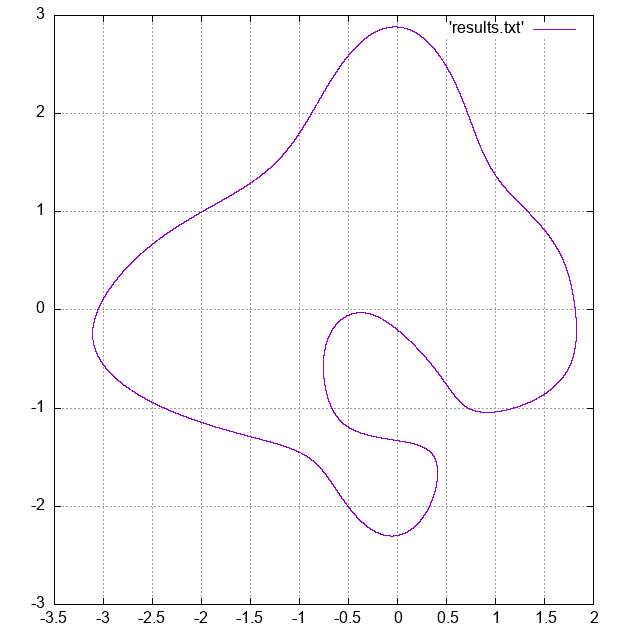
\includegraphics[width=0.35\textwidth]{YaremaTaras.png}
    \caption{Plot of the curve such that $f(C) = 0$}
    \label{fig:plot}
\end{figure}

\bibliographystyle{plain}
\bibliography{YaremaTaras}

\end{document}
